\chapter{Emission model}
\label{cha:emission_model}

In this chapter, a sandwich layering model is analyzed and compared using two different methods. An extension of multiple layers is followed. 

\section{Sandwich emission model}
\label{sec:sandwich}
Considering the case of three layers, with the air on the top, snow layer in the middle and ice at the bottom. Two methods are applied to show the effect of dielectric constants on upwelling brightness temperature above the top layer.

\subsection{Method used by MEMLS}
\label{sandwich_memls}
\begin{figure}[!h]
  \centering
 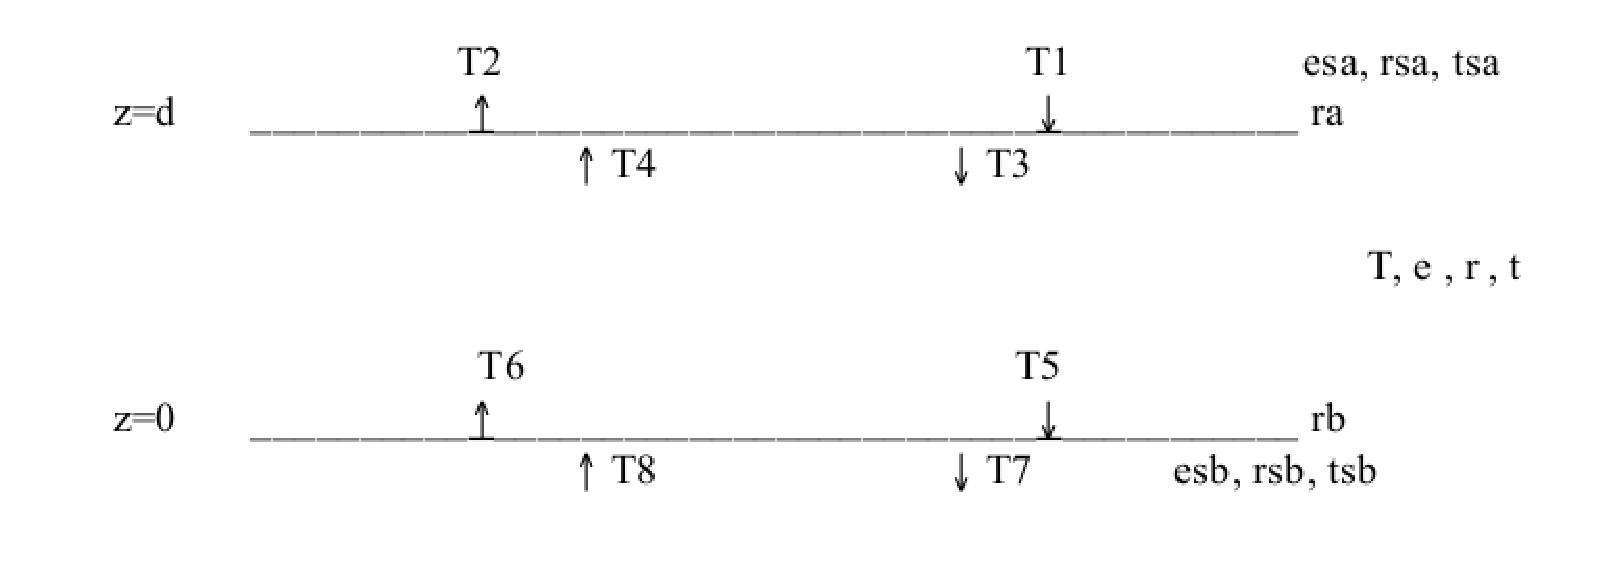
\includegraphics[scale=0.5]{sandwich.eps} 
  \caption{Sandwich model of a plane parallel snow slab with thickness d, illuminated by brightness temperature T1 from above and by T8 from below, emitting T2 upwards and T7 downwards (Source: Fig 1 in Note 1)}
\label{fig:sandwich}
\end{figure}
As Fig. \ref{fig:sandwich} shows, air locates above $z=d$ plane and the ice locates beneath the $z=0$ plane. The snow slab is at the middle. The emissivity of  the snow layer has an internal emissivity of $e$, transmissivity of $t$ and reflectivity of $r$. And $T$ is the physical temperature of snow layer. Th reflectivity at air-snow and snow-ice interface is $r_a$ $r_b$ respectively. $esa,rsa,tsa$ is the total emissivity ,reflectivity and total transmissivity when illuminated from above. And $esb,rsb,tsb$ is the total emissivity ,reflectivity and total transmissivity when illuminated from below. 
Assuming T is zero, the internal brightness temperature relates with the external temperature as the following:
\begin{equation*}
  \label{eq:sandwich}
\begin{split}
T2&=raT1+(1-ra)T4;\\
T3&=(1-ra)T1+raT4;\\
T4&=rT3+tT6;\\
T5&=tT3+rT6;\\
T6&=rbT5+(1-rb)T8;\\
T7&=(1-rb)T5+rbT8;\\
\end{split}
\end{equation*}

On the case of $T\neq0$, the emission contribution should be included. Now the brightness temperature $T_2$ can be computed as: 
\begin{equation*}
  T_2 = rsaT_1+esaT+tsT_8
\end{equation*}
$T$ is the physical temperature of snow. $rsa$ can be computed using the $e,r,t$ of each layer and the interface reflectivity $rsa$ and $rsb$:
\begin{equation*}
  \begin{split}
    &rsa=ra+(1-ra)^2roa/(1-ra.roa)\\
    &rsb=rb+(1-rb)^2rob/(1-rb.rob)\\
&ts=tsa=tsb=t(1-ra)(1-rb)/((1-r.ra)(1-rb)-ra.rb.t^2)
  \end{split}
\end{equation*}
where $roa$ and $rob$ is:
\begin{equation*}
  \begin{split}
    roa=r+rb.t^2/(1-r.rb)\\
    rob=r+ra.t^2/(1-r.ra)\\
  \end{split}
\end{equation*}

The refractive index $n=n'+in''$ can be calculated from the dielectric constant $\epsilon = \epsilon_1+i\epsilon_2$:
\begin{equation*}
\begin{split}
  n'&=\sqrt{\frac{\sqrt{\epsilon_1^2+\epsilon_2^2}+\epsilon_1}{2}}\\
  n''&=\sqrt{\frac{\sqrt{\epsilon_1^2+\epsilon_2^2}-\epsilon_1}{2}}
\end{split}
\end{equation*}
When $\epsilon_1\gg\epsilon_2$, $n=n'=\sqrt{\epsilon_1}$.\\

The interface reflectivity of horizontal and vertical polarization  then can be found by the Snell's law and Fresnel equation. At the air-snow interface,
\begin{equation*}
\begin{split}
  ra_h &= \left[\frac{n_1cos(\theta_i)-n_2cos(\theta_t)}{n_1cos(\theta_i)+n_2cos(\theta_t)}\right]
       = \left[\frac{n_1cos\theta_1-n_2\sqrt{1-(\frac{n_1}{n_2}sin\theta_1)^2}}{n_1cos\theta_1+n_2\sqrt{1-(\frac{n_1}{n_2}sin\theta_1)^2}}\right]^2\\
  ra_v &= \left[\frac{n_1cos(\theta_t)-n_2cos(\theta_i)}{n_1cos(\theta_t)+n_2cos(\theta_i)}\right]
       = \left[\frac{n_2cos\theta_1-n_1\sqrt{1-(\frac{n_1}{n_2}sin\theta_1)^2}}{n_2cos\theta_1+n_1\sqrt{1-(\frac{n_1}{n_2}sin\theta_1)^2}}\right]^2
\end{split}
\end{equation*}
And at the snow-ice interface, $n_1$ and $n_2$ is the refractive index of snow and ice respectively. And the incidental angle $\theta_2$ is:
\begin{equation*}
 \theta_2=\arcsin{\frac{sin\theta_1}{n_{snow}}}
\end{equation*}
\begin{figure}[hbp]
  \centering
   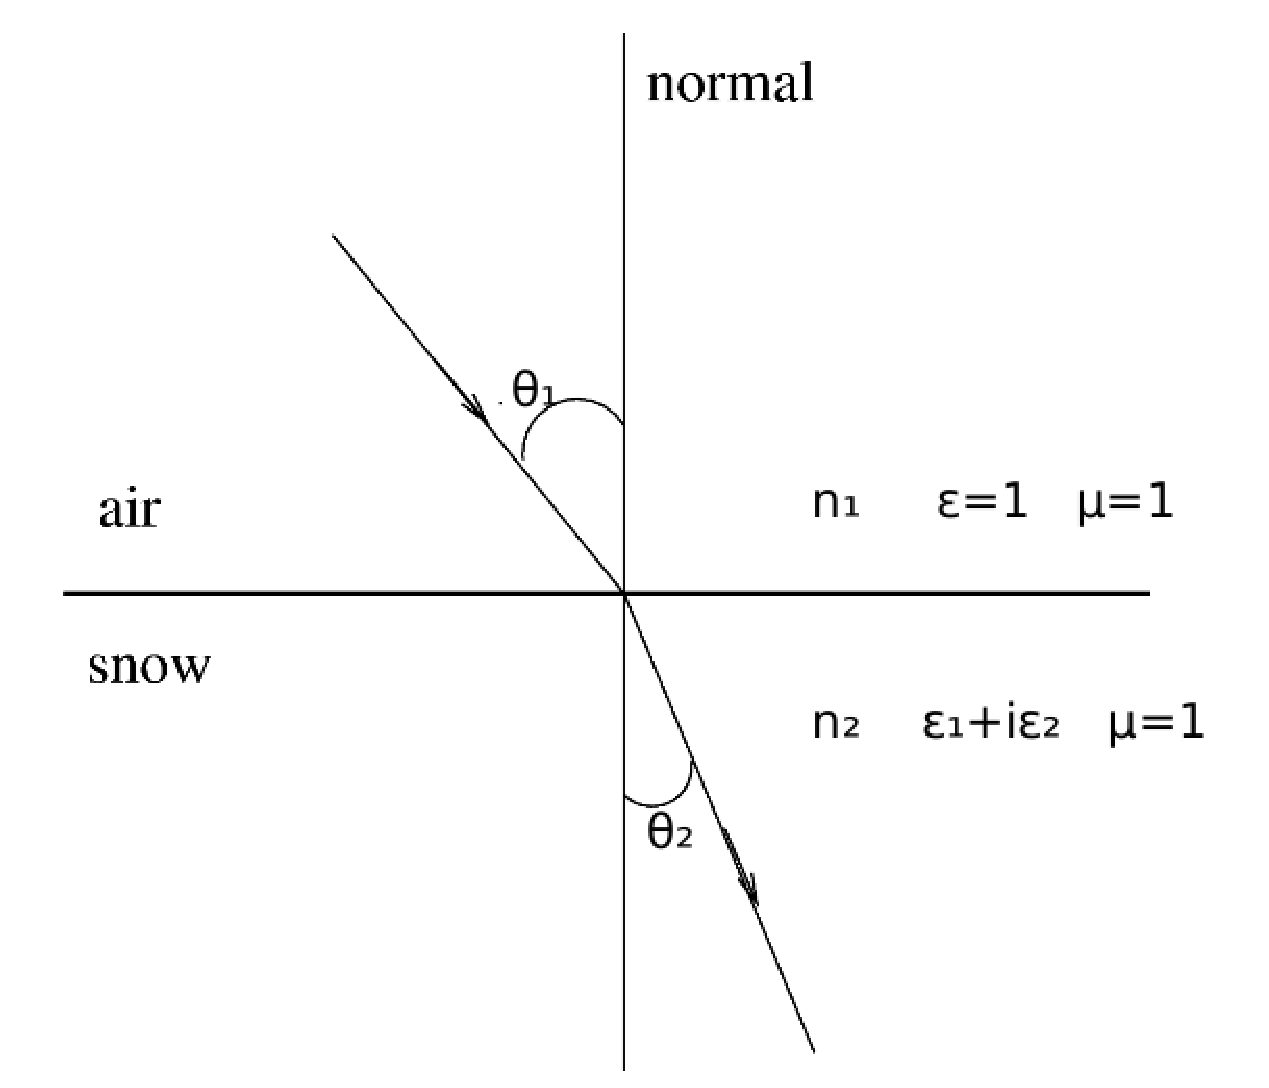
\includegraphics[scale=0.45]{snell.eps} 
  \caption{Reflection at air-snow interface}
  \label{fig:snell}
\end{figure}
As for the layer internal parameters, the internal radiative-transfer equation describes how radiation (T4 to T6 in Fig \ref{fig:sandwich}) is modified when it propagates over a path.  The  radiance is increased by emission and reduced by absorption. Considering the 6-flux radiative model showed in figure Fig \ref{fig:6flux}. All the horizontal fluxes are the same. The vertical fluxes is: \\
\begin{equation*}
\begin{split}
    \frac{dT_1}{dz}\vert cos\theta \vert &={\gamma}_a(T_1-T)+\gamma_b(T_1-T_2)\\
    \frac{dT_2}{dz}\vert cos\theta \vert &=-{\gamma}_a(T_2-T)-\gamma_b(T_1-T_2)\\
\end{split}
\end{equation*}
where $\gamma_a$ is the absorption coefficients and $\gamma_b$ is the scattering coefficients. 

\begin{figure}[!hbp]
  \centering
   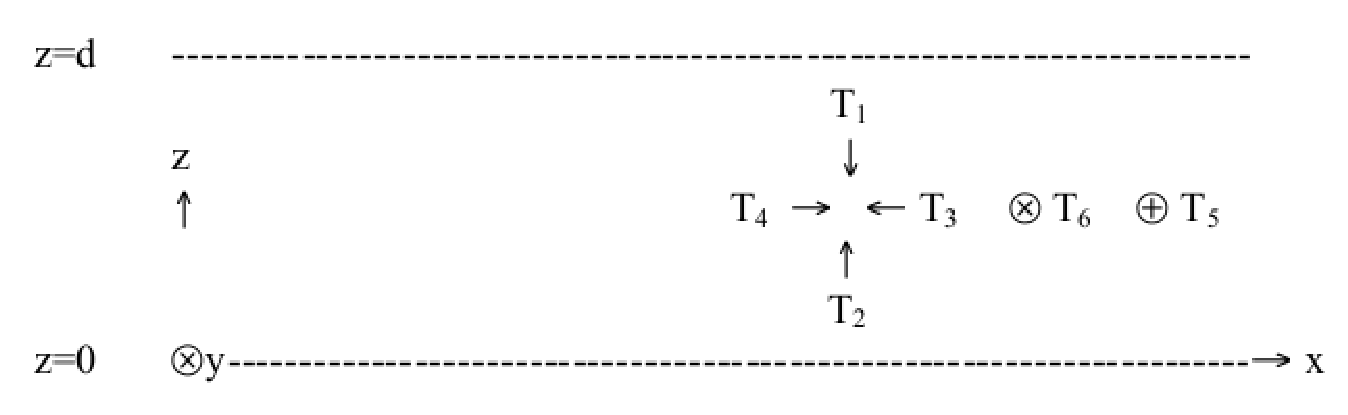
\includegraphics[scale=0.5]{6flux.eps} 
  \caption{Six fluxes inside the snow layer(Source: Note 2 Fig.1)}
  \label{fig:6flux}
\end{figure}

The total reflectivity, emissivity and transmissivity can be calculated by $\gamma_a$ and $\gamma_b$:
\begin{equation*}
\begin{split}
r&=\frac{r_0(1-{t_0}^2)}{1-{r_0}^2{t_0}^2}\\
t&=\frac{t_0(1-{r_0}^2)}{1-{r_0}^2{t_0}^2}\\
r_0&=\frac{\gamma_b}{\gamma_a+\gamma_b+\gamma}\\
\gamma&=\sqrt{\gamma_a(\gamma_a+2\gamma_b)}\\
t_0&=e^{-{\gamma}d/\vert cos\theta\vert}  
\end{split}  
\end{equation*}
where $\gamma$ is the damping coefficient.

\subsection{Impedance matching}
\begin{figure}[!hbp]
  \centering
   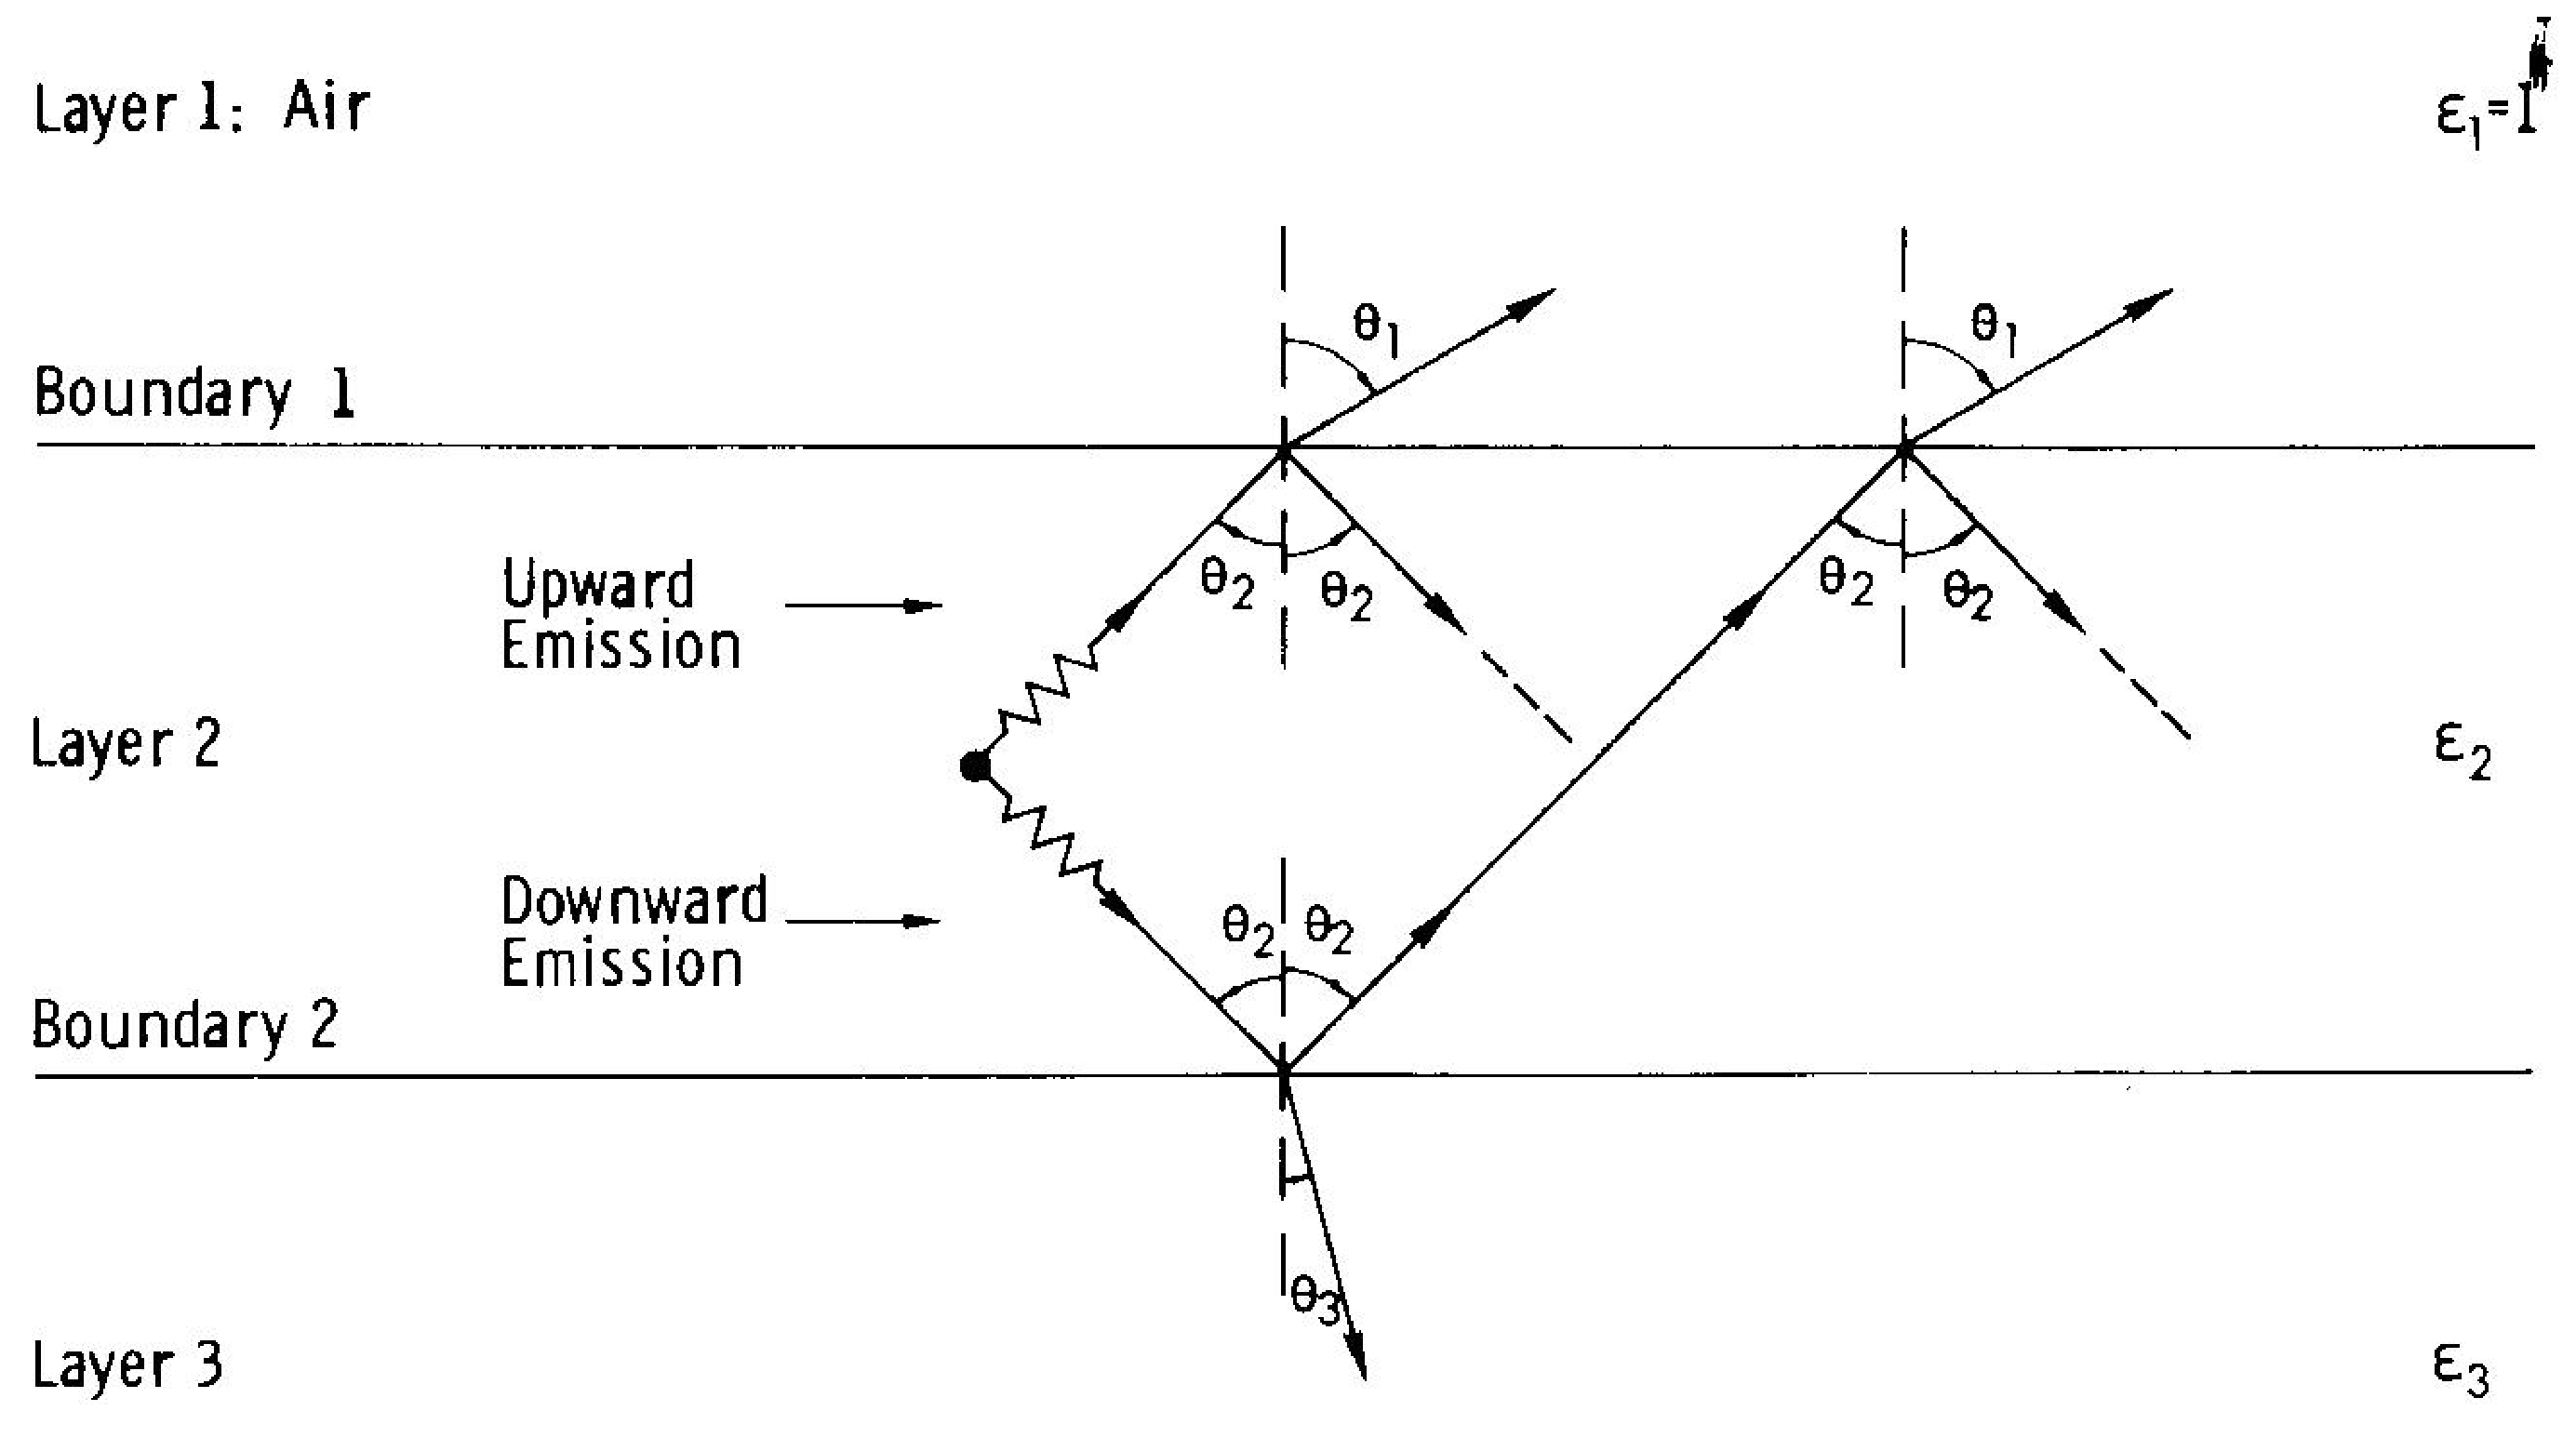
\includegraphics[scale=0.2]{incoherent_layer.eps} 
  \caption{Emission by layer 2 into layer 1 (Source: Ulaby. Microwave remote sensing. vol1. Fig 4.24)}
  \label{fig:incoherent_layer}
\end{figure}
Another way to analyze the sandwich model is by means of impedance matching. Considering the incoherent case where the profile has a continuous dielectric constant, the upwelling brightness temperature is contributed from emission from snow and ice layer:
\begin{equation*}
  T_B = T_{B2}+T_{B3}
\end{equation*}
And the emission from each layer is the sum of the downward emitted radiation $T_D$ and upward emitted $T_D$ which is illustrated on Fig.\ref{fig:incoherent_layer}. Including all the multiple reflections as showed in Fig.\ref{fig:incoherent}, the contributions from snow and ice into air is computed.
\begin{figure}[!hbp]
  \centering
   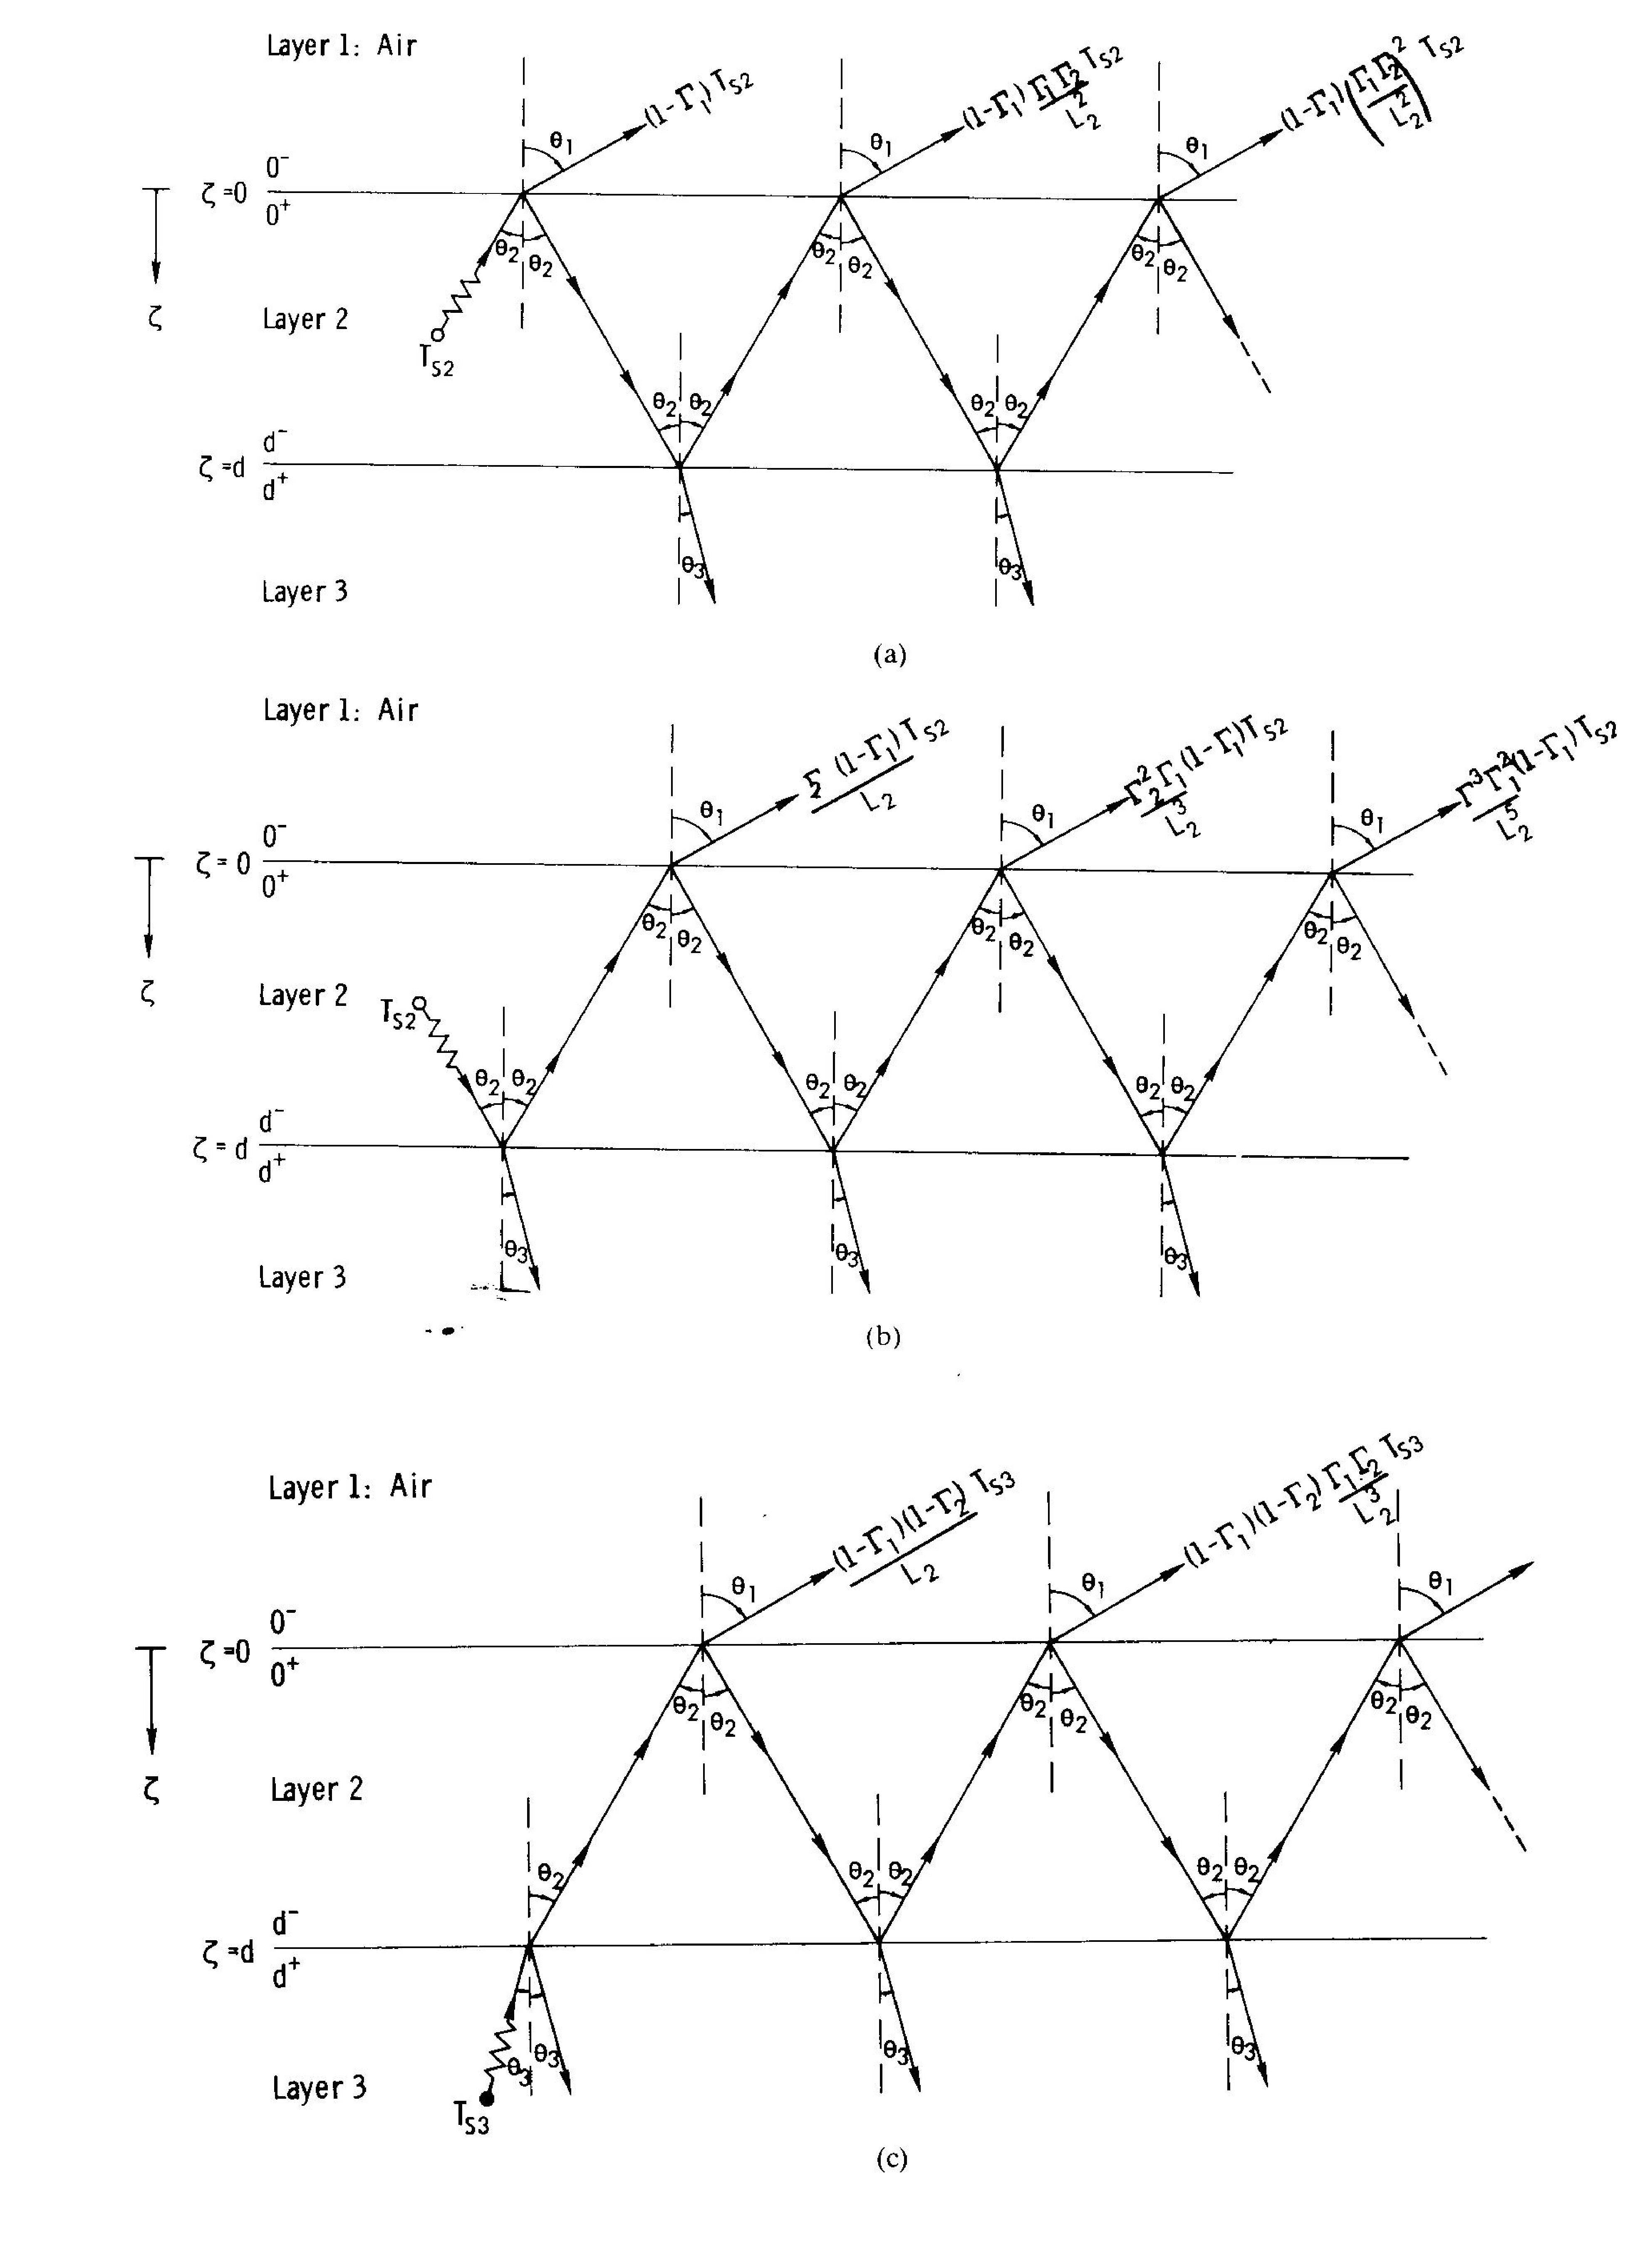
\includegraphics[scale=0.2]{incoherent_Tb.eps} 
  \caption{(a) Upward emission from snow layer $T_{2U}$;(b) Downward emission from snow layer $T_{2D}$;(c) Downward emission from ice layer $T_{3U}$(Source: Ulaby. Microwave remote sensing. vol1. Fig 4.25)}
  \label{fig:incoherent_Tb}
\end{figure}

The upward emitted radiation from snow layer is:
\begin{equation*}
\begin{split}
  T_{2U} &= (1-\Gamma_1)T_{S2}+(1-\Gamma_1)\frac{\Gamma_1\Gamma_2}{L_2^2}T_{S2}+....\\
         &= (1-\Gamma_1)T_{S2}[1+x+x^2+....]
\end{split}
\end{equation*}
where $x=\frac{\Gamma_1\Gamma_2}{L_2^2}$
The reflectivity at the air-snow and snow-ice interface $\Gamma_1$ $\Gamma_2$ is decided by the intrinsic impedance. 
\begin{equation*}
  \Gamma_1 = \lvert\frac{Z_{snow}-Z_{air}}{Z_{snow}+Z_{air}}\rvert^2\\
  \Gamma_2 = \lvert\frac{Z_{ice}-Z_{snow}}{Z_{ice}+Z_{snow}}\rvert^2\\
\end{equation*}
The intrinsic impedance of each layer is:
\begin{equation*}
  \begin{split}
    Z_h&=\sqrt{\frac{\mu_r}{\epsilon_r}}cos\theta \\
    Z_v&=\sqrt{\frac{\mu_r}{\epsilon_r}}sec\theta
  \end{split}
\end{equation*}
The loss factor of snow layer $L_2$ is:
\begin{equation*}
  L_2=e^{2\alpha dsec\theta_2}
\end{equation*}
where $\alpha=\frac{2\pi}{\lambda_0}$|Im$\sqrt{\epsilon}$| and $d$ is the thickness of snow layer.
The total energy received at air-snow interface by snow layer is:
\begin{equation*}
  T_{S2}=(1-a_2)T_2(1-\frac{1}{L_2})
\end{equation*}
where $T_2$ is the physical temperature and $a_2$ is the single-scattering albedo.
Because $\Gamma_1$ $\Gamma_2$ is smaller than one and loss factor is larger than one, $x<1$, the sum has a closed form:
\begin{equation*}
  T_{2U} = \frac{(1-\Gamma_1)T_{S2}}{1-\Gamma_1\Gamma_2/L_2^2}
\end{equation*}
The downward emitted radiation from snow layer is:
\begin{equation*}
\begin{split}
  T_{2D} &= \frac{\Gamma_2(1-\Gamma_1)T_{S2}}{L_2}+\frac{\Gamma_2^2\Gamma_1(1-\Gamma_1)T_{S2}}{L_2^3}+\frac{\Gamma_2^3\Gamma_1^2(1-\Gamma_1)T_{S2}}{L_2^5}+...\\
         &= \frac{\Gamma_2(1-\Gamma_1)T_{S2}}{L_2}(1+x+x^2+...)
\end{split}
\end{equation*}
Likewise, the closed form is:
\begin{equation*}
  T_{2D} = \frac{\Gamma_2(1-\Gamma_1)T_{S2}}{L_2(1-\Gamma_1\Gamma_2/L_2^2)}
\end{equation*}
The radiation contribution from ice only includes upward emitted radiation assuming that the ice has semi-infinite depth in which case
\begin{equation*}
  T_{S3} = T_3
\end{equation*}
where $T_3$ is the physical temperature of ice.
The radiation contribution from ice is then given as:
\begin{equation*}
  T_{B3}=\frac{(1-\Gamma_1)(1-\Gamma_2)T_3}{L_2(1-\Gamma_1\Gamma_2/L_2^2)}
\end{equation*}
Summing all the contribution together, the upwelling brightness temperature at the air-snow interface is:
\begin{equation*}
  T_B=\left(\frac{1-\Gamma_1T_3}{1-\Gamma_1\Gamma_2/L_2^2}\right)\left[\left(1+\frac{\Gamma_2}{L_2}\right)\left(1-\frac{1}{L_2}\right)(1-a)T_2+\frac{1-\Gamma_2}{L_2}T_3\right]
\end{equation*}
\subsection{Comparison}
Excluding the scattering in the above two methods and assuming the sky radiance is zero which leads to $\gamma=2\alpha$ $T_1=0$ and $a_2=0$, it can be derived that:
\begin{equation*}
\begin{split}
  TB_{MEMLS} &= \left(\frac{1-\Gamma_1T_3}{1-\Gamma_1\Gamma_2/L_2^2}\right)\left[(1+\Gamma_2t)(1-t)T_2+t(1-T_2)T_3\right]\\
            &= TB_{impedance}
\end{split}
\end{equation*}
where $t=t_0=e^{-\gamma dsec\theta_2}$.
Fig. \ref{fig:2layer} is curve of brightness temperature by the permittivity of the snow. As expected, the two methods give the identical curve. The dielectric of ice is $\epsilon=3.2+i0.5$. The depth of the snow layer is 20cm. The physical temperature of snow and ice layer is 250K and 270K respectively. The permittivity of the snow varies from 1.4 to 3.2. Upwelling brightness temperature reduces with larger permittivity which shows the reflection happened at the snow-ice interface is more dominant of the radiation contribution. The decreasing value of H channel is about 40K within the permittivity range while the V channel hardly changes with the permittivity.
\begin{figure}[hbp]
  \centering
   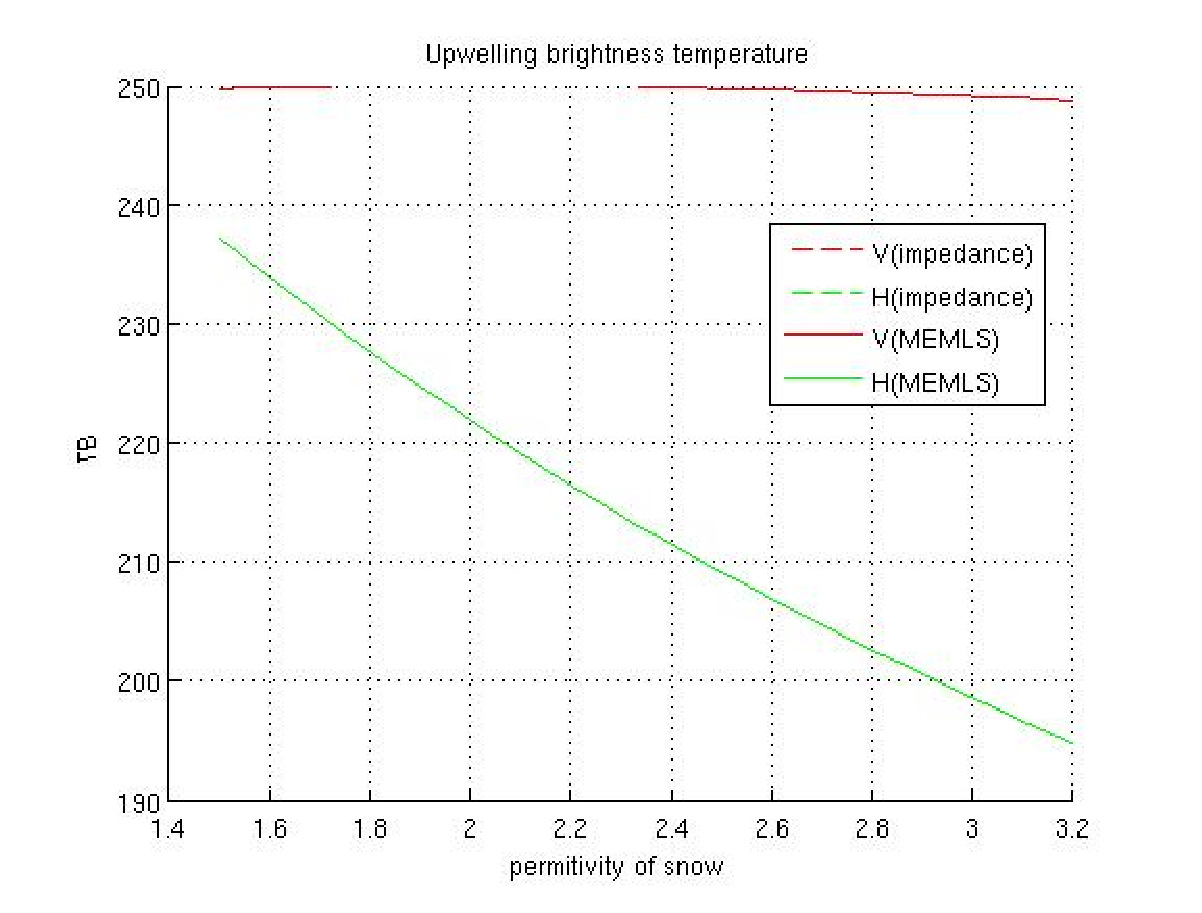
\includegraphics[scale=0.5]{2layer.eps} 
  \caption{Upwelling temperature vs. permittivity of snow with impedance matching and MEMLS method }
  \label{fig:2layer}
\end{figure}
\clearpage

\section{Multiple layers}
\label{sec:mult}
\begin{figure}[hbp]
  \centering
   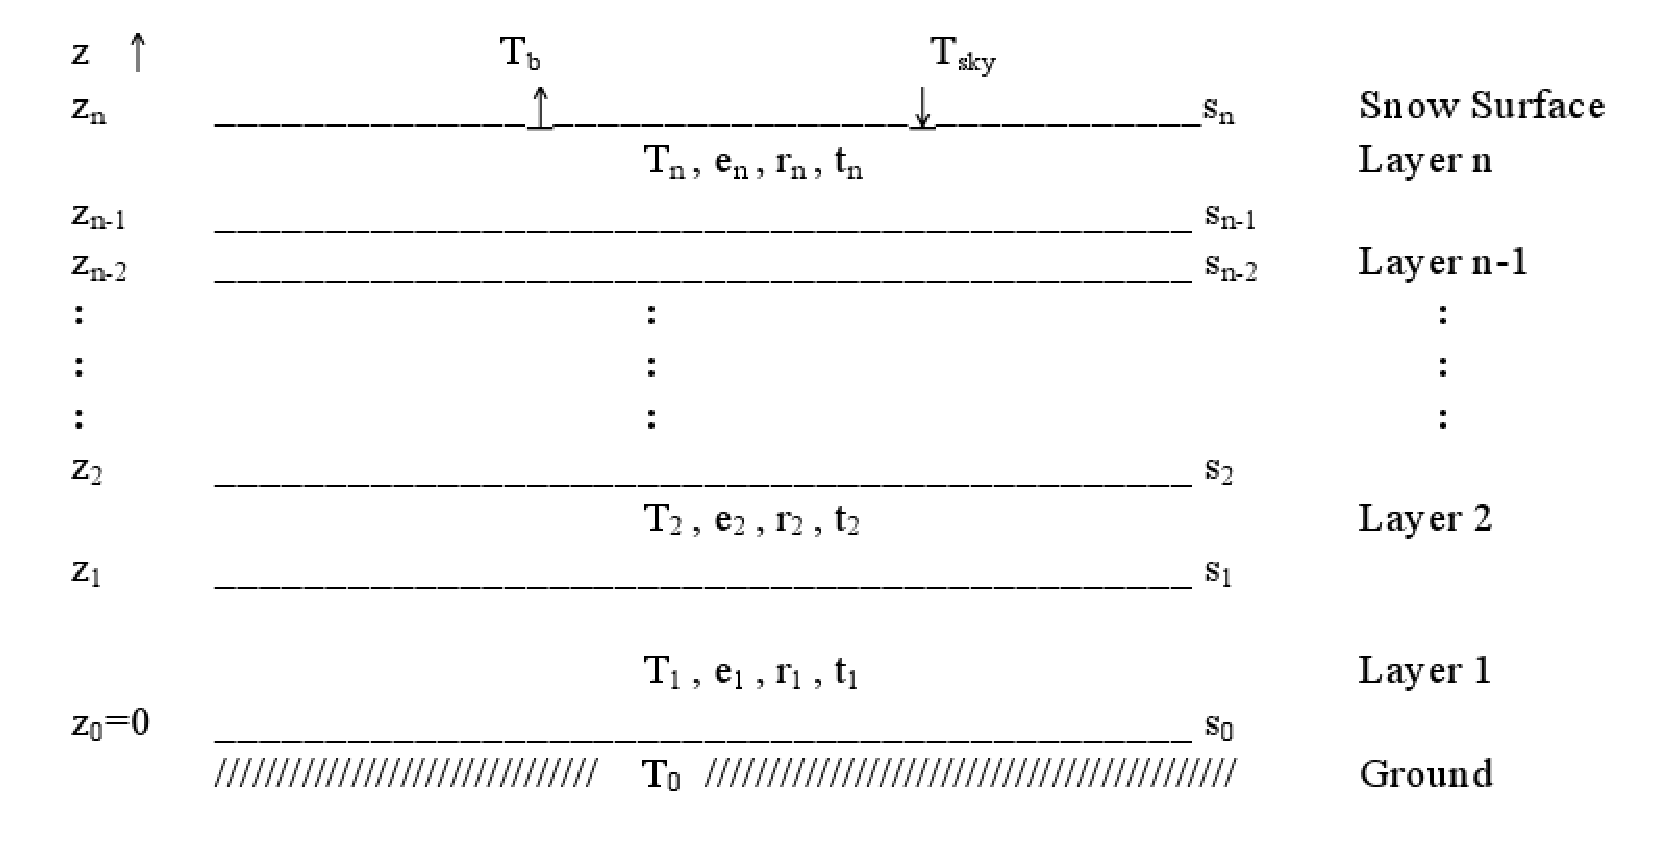
\includegraphics[scale=0.5]{multilayers.eps} 
  \caption{n layers structure. (Source: MEMLS Note.6s Fig.1)}
  \label{fig:mul}
\end{figure}
The sandwich model can be extended to multiple layers as showed in Fig. \ref{fig:mul} either by MEMLS way or by impedance matching way. 
\subsection{Method used by MEMLS}
\label{sec:mul_memls}
MEMLS uses an iteration method and treats the parameters in matrix to give an extension to the multiple layers. For each layer, it is characterized by the layer parameters as showed in Fig.\ref{fig:onelayer_memls}.
\begin{figure}[hbp]
  \centering
   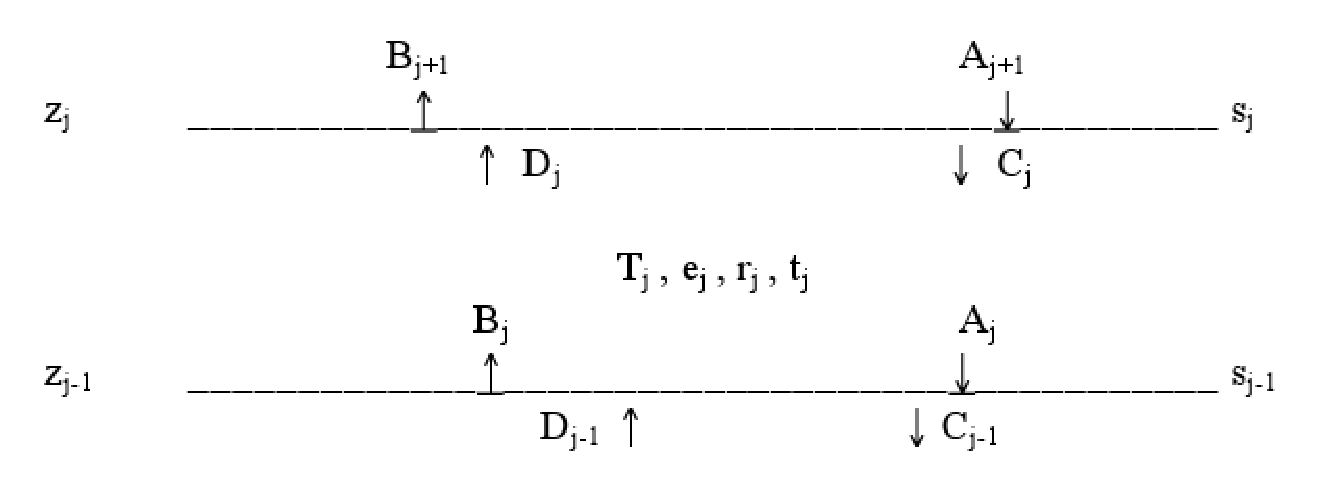
\includegraphics[scale=0.5]{onelayer.eps} 
  \caption{The parameters of a selected layer. (Source: MEMLS Note.6s Fig.1)}
  \label{fig:onelayer_memls}
\end{figure}
At the boundaries, the brightness temperature is related by:
\begin{equation*}
\begin{split}
  A_j &= r_jB_j +t_jC_j+e_jT_j\\ 
  B_j &= s_{j-1}A_j +(1-s_{j-1})D_{j-1}\\ 
  C_j &= (1-s_j)D_{j+1}+s_jD_j\\ 
  D_j &= t_jB_j +r_jC_j+e_jT_j\\ 
  D_0 &= T_0\\
  A_{n+1} &= T_{sky}\\
  T_b &= (1-s_n)D_n+s_nT_{sky}
\end{split}
\end{equation*}
where $j$ is from 1 to $n$. Eliminating $B_j$ and $C_j$, $A_j$ and $D_j$ is expressed as:
\begin{equation*}
  \begin{split}
      A_j &= r_j[s_{j-1}A_j+(1-s_{j-1})D_{j-1}] +t_j[(1-s_j)A_{j+1}+s_jD_j]+e_jT_j\\
      D_j &= t_j[s_{j-1}A_j+(1-s_{j-1})D_{j-1}] +r_j[(1-s_j)A_{j+1}+s_jD_j]+e_jT_j
  \end{split}
\end{equation*}
Witting in form of matrix:
\begin{equation*}
\begin{split}
\bf{A}&=\bf{M_1}.\bf{A}+\bf{M_2}\bf{D}+\bf{E}\\  
\bf{A}&=\bf{M_3}.\bf{A}+\bf{M_4}\bf{D}+\bf{F}
\end{split}
\end{equation*}
Then the upwelling brightness temperature at each layer interface can be achieved by:
\begin{equation*}
    \bf{D} = (\bf{I} -\bf{M_5})^{-1}.(\bf{M_3}.(\bf{I}-\bf{M_1})^{-1}.\bf{E}+\bf{D}) 
 \end{equation*}
where 
\begin{equation*}
  \bf{D}=\bf{M_3}.{(\bf{I}-\bf{M_1})^{-1}.\bf{M_2}}+\bf{M_4}
\end{equation*}.
If there are 2 layers presented, matrix $\bf{M_1,M_2,M_3,M_4}$ is:
\[ \bf{M_1} = \left( \begin{array}{cc}
r_1s_0 & t_1(1-s_1) \\
0      & r_2s_1     \end{array} \right) \] 

\[ \bf{M_2} = \left( \begin{array}{cccc}
t_1s_1 & 0  \\
r_2(1-s_1) & t_2s_s \end{array} \right) \] 

\[ \bf{M_3} = \left( \begin{array}{cccc}
t_1s_0 & r_1(1-s_1) \\
0      & t_2s_1     \end{array} \right) \] 


\[ \bf{M_4} = \left( \begin{array}{cccc}
r_1s_1 & 0  \\
t_2(1-s_1)      & r_2s_s   \end{array} \right) \] 

\[ \bf{E} = \left( \begin{array}{l}
e_1T_1 + r_1(1-s_0)T_0\\
e_4T_2 + t_2(1-s_1)T_{sky} \end{array} \right) \] 

\[ \bf{F} = \left( \begin{array}{l}
e_1T_1 + t_1(1-s_0)T_0\\
e_2T_2 + r_2(1-s_1)T_{sky} \end{array} \right) \] 
\subsection{Impedance matching}
\label{sec:mul_impedance}
Considering the same layer structure as Fig \ref{fig:mul} but with inverse layer numbering ie increase from top to bottom, for the  \sl{i}th layer, the radiation contribution of the upward emitted and the downward emitted into the top layer can be derived as:
\begin{equation*}
\begin{split}
T_{iU} &= \prod_{1\le l\le i-1}(1-\Gamma_l)T_{Si}\frac{1}{\prod_{2\le l\le i-1}L_l}\prod_{2\le l\le i}(\frac{1}{1-\Gamma(l-1)\Gamma(l)/L_l^2})\\ 
T_{iD} &= \prod_{1\le l\le i-1}(1-\Gamma_l)T_{Si}\Gamma_l\frac{1}{\prod_{2\le l\le i}L_l}\prod_{2\le l\le i}(\frac{1}{1-\Gamma(l-1)\Gamma(l)/L_l^2})  
\end{split}
\end{equation*}
where i is from 2 to n. And 
\begin{equation*}
  T_{Si}= (1-a_i)T_i(1-\frac{1}{L_i})
\end{equation*}
\subsection{Comparison}               


%%% Local Variables: 
%%% mode: latex
%%% TeX-master: "main"
%%% End: 
